%=======================================================
% CHAPTER 3: QUASI-CYCLIC SYNDROME DECODING — THE RESOLUTION
%=======================================================

\begin{frame}[plain]
  \begin{center}\bfseries\centering
    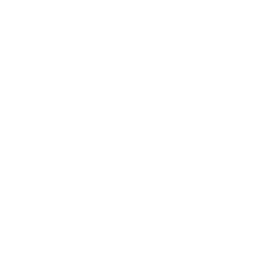
\includegraphics[scale=1]{assets/branding/opa0}
    \vspace{-5.75cm}\\
    {\adjustbox{scale=1.4}{\color{TealDarkCyan}\;IV.\;Quasi-Cyclic Syndrome Decoding}}
    \vspace{.25cm}
    \begin{minipage}{.78\textwidth}
      \scriptsize\color{Ink}
      \textbf{Big picture.}\;
      Quasi-cyclic structure compresses public keys from megabytes to kilobytes
      while keeping the essential hardness of SDP — but it opens new attack surfaces.\\[.2cm]
      \textbf{Details to watch.}\;
      circulant matrix, QCSD, key compression, BIKE, HQC, DOOM attack, hardness hierarchy.
    \end{minipage}
    {\ }\vspace{2.1cm}\\
    \bigskip
  \end{center}
\end{frame}

%--- The engineering resolution ---
\begin{frame}{\textbf{IV. Quasi-Cyclic Syndrome Decoding}}{The Engineering Resolution}
\small
\begin{columns}[T,onlytextwidth]
\begin{column}{.50\textwidth}
\textcolor{TealDarkCyan}{\textbf{Problem (Act III)}}
\begin{itemize}
  \item SDP is NP-complete and quantum-resistant.
  \item But random $\mat H$ forces $O(n^2)$-bit public keys.
  \item Classic McEliece: $261\,\text{KB}$ — impractical for many applications.
\end{itemize}
\end{column}
\begin{column}{.46\textwidth}
\textcolor{TealDarkCyan}{\textbf{Resolution (Act IV)}}
\begin{itemize}
  \item Add \emph{circulant} structure: each block described by one polynomial.
  \item Key size drops to $O(n)$ bits — a factor $\approx n/2$ reduction.
  \item Hardness \emph{inherited} from SDP; new attacks studied carefully.
\end{itemize}
\end{column}
\end{columns}
\bigskip
\begin{center}
\begin{tikzpicture}[node distance=.7cm]
  \node[process red,minimum width=3.0cm,align=center] (sdp)
    {SDP: NP-complete\\large keys $O(n^2)$};
  \node[process blue,right=1.2cm of sdp,minimum width=3.0cm,align=center] (qc)
    {QC structure\\circulant blocks};
  \node[process amber,right=1.2cm of qc,minimum width=3.0cm,align=center] (qcsd)
    {QCSD: hard\\compact keys $O(n)$};
  \node[process,right=1.2cm of qcsd,minimum width=2.6cm,align=center] (pqc)
    {BIKE / HQC\\NIST PQC};
  \draw[flow red]   (sdp) -- (qc);
  \draw[flow blue]  (qc)  -- (qcsd);
  \draw[flow amber] (qcsd)-- (pqc);
\end{tikzpicture}
\end{center}
\end{frame}

%--- Circulant matrices ---
\begin{frame}{\textbf{IV. Quasi-Cyclic Syndrome Decoding}}{Circulant Matrices: The Building Block}
\small
\defbox[Circulant matrix]{
$\mathrm{circ}(h_0,\ldots,h_{m-1})\in\F_q^{m\times m}$: each row is a cyclic shift of the row above.
\[
  \mat C = \begin{pmatrix}
    h_0 & h_1 & \cdots & h_{m-1} \\
    h_{m-1} & h_0 & \cdots & h_{m-2} \\
    \vdots & & \ddots & \vdots \\
    h_1 & h_2 & \cdots & h_0
  \end{pmatrix}
\]
}
\begin{columns}[T,onlytextwidth]
\begin{column}{.54\textwidth}
\begin{itemize}
  \item $\mat C$ corresponds to $h(X)=\sum h_i X^i\in R_m=\F_q[X]/(X^m-1)$.
  \item $\mathrm{circ}(h)\cdot\mathrm{circ}(g) = \mathrm{circ}(h\cdot g\bmod X^m-1)$.
  \item Entire $m\times m$ matrix compressed to $m$ bits.
  \item Arithmetic in $R_m$ is fast: NTT-based multiplication in $O(m\log m)$.
\end{itemize}
\end{column}
\begin{column}{.42\textwidth}
\begin{center}
\begin{tikzpicture}[scale=.72]
  % Left circulant H0
  \draw[TealDarkCyan,thick,fill=TealDarkCyan!8] (0,0) rectangle (2.6,2.2);
  \node[tiny label,TealDarkCyan] at (1.3,2.45) {$\mat H_0=\mathrm{circ}(h_0)$};
  \foreach \d in {0,...,3}{
    \pgfmathsetmacro{\y}{0.5+0.5*\d}
    \pgfmathsetmacro{\xs}{0.55*\d}
    \draw[TealDarkCyan!50,line width=1.4pt] (\xs,\y) -- (\xs+0.5,\y);
  }
  \node[tiny label,AccentCyan!80] at (1.3,1.1) {circulant};
  % Right circulant H1
  \draw[BlueCode,thick,fill=BlueCode!7] (2.9,0) rectangle (5.5,2.2);
  \node[tiny label,BlueCode] at (4.2,2.45) {$\mat H_1=\mathrm{circ}(h_1)$};
  \foreach \d in {0,...,3}{
    \pgfmathsetmacro{\y}{0.5+0.5*\d}
    \pgfmathsetmacro{\xs}{2.9+0.55*\d}
    \draw[BlueCode!50,line width=1.4pt] (\xs,\y) -- (\xs+0.5,\y);
  }
  \node[tiny label,BlueCode!80] at (4.2,1.1) {circulant};
  \draw[<->,Ink!55,line width=.6pt] (-0.3,0)--(-0.3,2.2)
    node[midway,left,tiny label]{$m$};
  \draw[<->,Ink!55,line width=.6pt] (0,-0.4)--(5.5,-0.4)
    node[midway,below,tiny label]{$n=2m$ (all described by 2 polynomials)};
\end{tikzpicture}
\end{center}
\end{column}
\end{columns}
\end{frame}

%--- QCSD definition ---
\begin{frame}[shrink=5]{\textbf{IV. Quasi-Cyclic Syndrome Decoding}}{The QCSD Problem}
\defbox[Quasi-Cyclic Syndrome Decoding (QCSD)]{
\textbf{Input:}\; block-circulant $\mat H=[\mat H_0\mid\cdots\mid\mat H_{\ell-1}]\in\F_q^{m\times\ell m}$,
$\mat H_i=\mathrm{circ}(h_i)$,\; syndrome $\vect s\in\F_q^m$,\; weight $w$.\\[4pt]
\textbf{Search:}\; find $\vect e=(\vect e_0|\cdots|\vect e_{\ell-1})\in\F_q^{\ell m}$ with
\[
  \sum_{i=0}^{\ell-1}\mat H_i\vect e_i^T = \vect s
  \quad\text{and}\quad \wt(\vect e)\le w.
\]
\textbf{Polynomial form:}\; find $e_i\in R_m$ with $\sum_i h_i e_i \equiv s\pmod{X^m-1}$ and $\sum_i\wt(e_i)\le w$.
}
\begin{columns}[T,onlytextwidth]
\begin{column}{.50\textwidth}
\textcolor{TealDarkCyan}{\textbf{Relation to SDP}}
\begin{itemize}
  \item QCSD is a structured instance of SDP.
  \item A QCSD solver implies an SDP solver (for this instance family).
  \item QC structure opens new algebraic and statistical attacks.
\end{itemize}
\end{column}
\begin{column}{.46\textwidth}
\textcolor{TealDarkCyan}{\textbf{Why it is still hard}}
\begin{itemize}
  \item No polynomial-time algorithm known.
  \item Algebraic attacks (Gröbner) fail at NIST parameters.
  \item NIST selected BIKE for standardization consideration.
\end{itemize}
\end{column}
\end{columns}
\end{frame}

%--- QC-MDPC codes ---
\begin{frame}{\textbf{IV. Quasi-Cyclic Syndrome Decoding}}{QC-MDPC Codes}
\small
\defbox[QC-MDPC Code (Misoczki et al., 2013)]{
A \textbf{Quasi-Cyclic Moderate Density Parity Check} code has parity-check matrix
$\mat H=[\mat H_0|\mat H_1]$ with $\mat H_i=\mathrm{circ}(h_i)$ and \emph{moderate} row weight $d_v\approx\sqrt{n}$.
}
\begin{columns}[T,onlytextwidth]
\begin{column}{.52\textwidth}
\textcolor{TealDarkCyan}{\textbf{Key features}}
\begin{itemize}
  \item Derived from LDPC philosophy but with higher weight than classical LDPC.
  \item Efficient probabilistic decoder: \textbf{iterative bit-flipping}.
  \item Security based on QCSD hardness, not on LDPC structure.
\end{itemize}
\textbf{Bit-flipping decoder.}\;
For each bit, count the parity checks it violates. Flip bits with the highest count. Iterate.
This is efficient but probabilistic — decoding failure rate $\delta_\mathrm{DFR}>0$.
\end{column}
\begin{column}{.44\textwidth}
\begin{center}
\begin{tikzpicture}[scale=.72]
  \draw[TealDarkCyan!40,fill=TealDarkCyan!5] (0,0) rectangle (2.2,1.8);
  \draw[BlueCode!40,fill=BlueCode!5]    (2.4,0) rectangle (4.6,1.8);
  \node[tiny label,TealDarkCyan] at (1.1,2.0) {$\mat H_0$};
  \node[tiny label,BlueCode] at (3.5,2.0) {$\mat H_1$};
  \foreach \x/\y in {.3/.4,.9/1.5,1.5/.8,.6/1.1,1.8/.3,
                     2.7/1.4,3.2/.5,3.8/1.0,4.3/1.6,2.9/.2}{
    \fill[TealDarkCyan!70] (\x,\y) circle (2pt);
  }
  \node[caption text,align=center,text width=4.5cm] at (2.3,-.55)
    {moderate weight: $d_v\approx\sqrt{n}$ ones per row};
\end{tikzpicture}
\end{center}
\end{column}
\end{columns}
\end{frame}

%--- BIKE ---
\begin{frame}[shrink=5]{\textbf{IV. Quasi-Cyclic Syndrome Decoding}}{BIKE: Bit Flipping Key Encapsulation}
\defbox[BIKE KEM (NIST PQC Round 4 finalist)]{
\textbf{Setup.}\; QC-MDPC code in $R_m^2$, $m$ prime, sparse $h_0,h_1\in R_m$ with $\wt=d_v$.

\textbf{Key generation.}\; Secret: $(h_0,h_1)$.  Public: $g=h_0^{-1}h_1\in R_m$.

\textbf{Encapsulation.}\;
Sample sparse $e_0,e_1\in R_m$ with $\wt(e_0)+\wt(e_1)=t$.
Ciphertext: $c=e_0+e_1\cdot g\in R_m$.

\textbf{Decapsulation.}\;
$c\cdot h_0 = e_0 h_0+e_1 h_1 = s$ (syndrome).
Run BGF bit-flipping decoder on $(s,h_0,h_1)$ to recover $(e_0,e_1)$.
}
\begin{columns}[T,onlytextwidth]
\begin{column}{.50\textwidth}
\textcolor{TealDarkCyan}{\textbf{Security}}
\begin{itemize}
  \item Breaking = solve QCSD on $(h_0,h_1)$, or find $(h_0,h_1)$ from $g$.
  \item Finding $(h_0,h_1)$ from $g=h_0^{-1}h_1$: \emph{polynomial factorization with weight constraints} in $R_m$ — no polynomial-time algorithm known.
\end{itemize}
\end{column}
\begin{column}{.46\textwidth}
\textcolor{TealDarkCyan}{\textbf{BIKE Level 1 parameters (128-bit)}}
\begin{center}
\renewcommand{\arraystretch}{1.1}
\begin{tabular}{ll}
  $m$ & 12323 \\
  $n=2m$ & 24646 \\
  $d_v$ & 71 \\
  $t$ & 134 \\
  Public key & 1541 bytes \\
  Ciphertext & 1573 bytes \\
\end{tabular}
\end{center}
\end{column}
\end{columns}
\end{frame}

%--- Decoding failure ---
\begin{frame}{\textbf{IV. Quasi-Cyclic Syndrome Decoding}}{Decoding Failure: A Critical Subtlety}
\small
\defbox[Decoding failure rate (DFR)]{
The BGF bit-flipping decoder fails with probability $\delta_\mathrm{DFR}$.
For BIKE Level 1: $\delta_\mathrm{DFR}\approx 2^{-128}$.
A non-zero DFR enables \emph{reaction attacks}.
}
\begin{columns}[T,onlytextwidth]
\begin{column}{.52\textwidth}
\textcolor{TealDarkCyan}{\textbf{The black-peg attack}}
\begin{itemize}
  \item Attacker submits chosen ciphertexts and observes decapsulation failures.
  \item Each failure leaks information about the secret key $(h_0,h_1)$.
  \item After polynomially many queries, the key can be recovered.
\end{itemize}
\textbf{Mitigation.}\;
BIKE uses a \emph{deterministic} BGF decoder variant.
The same ciphertext always decapsulates the same way, removing the oracle.
\end{column}
\begin{column}{.44\textwidth}
\begin{center}
\begin{tikzpicture}[scale=.74,transform shape,node distance=.52cm]
  \node[process]              (enc) {encapsulate\\$(e_0,e_1)$};
  \node[process blue,below=of enc]  (synd) {syndrome\\$s\in R_m$};
  \node[process amber,below=of synd](bgf) {BGF bit-flip\\decoder};
  \node[process red,below=of bgf]   (check){$(e_0',e_1')=?$};
  \node[process,below=of check,fill=GoodGreen!10,draw=GoodGreen!70] (ok) {accept};
  \node[process red,right=.8cm of check,minimum width=1.4cm,align=center]
    (fail){DFR\\$2^{-128}$};
  \draw[flow]       (enc)  -- (synd);
  \draw[flow blue]  (synd) -- (bgf);
  \draw[flow amber] (bgf)  -- (check);
  \draw[flow,GoodGreen!80] (check)--node[right,tiny label]{yes}(ok);
  \draw[flow red]   (check.east)--node[above,tiny label]{no}(fail);
\end{tikzpicture}
\end{center}
\end{column}
\end{columns}
\end{frame}

%--- HQC ---
\begin{frame}{\textbf{IV. Quasi-Cyclic Syndrome Decoding}}{HQC: Hamming Quasi-Cyclic}
\small
\defbox[HQC KEM (NIST PQC Round 4 alternate)]{
\textbf{Setup.}\; Work in $R_n=\F_2[X]/(X^n-1)$, $n$ prime.  Choose random $h\in R_n$.

\textbf{Key generation.}\;
Secret: sparse $x,y\in R_n$.\;
Public: $s=x+yh\in R_n$.

\textbf{Encapsulation.}\;
Sample sparse $r_1,r_2,e\in R_n$.
Ciphertext: $(\vect u,\vect v)=(r_1+r_2 h,\;mr_2+sr_1+e)$.

\textbf{Decapsulation.}\;
$\vect u\cdot y \approx \vect v\cdot r_2/r_2$ (inner product extraction), then decode the inner BCH or RS code.
}
\begin{columns}[T,onlytextwidth]
\begin{column}{.50\textwidth}
\textcolor{TealDarkCyan}{\textbf{HQC Level 1 (128-bit)}}
\begin{center}
\renewcommand{\arraystretch}{1.1}
\begin{tabular}{ll}
  $n$ & 17669 \\
  Weight of $x,y$ & 66 \\
  Weight of $r_1,r_2,e$ & 75 \\
  Public key & 2249 bytes \\
  Ciphertext & 4481 bytes \\
\end{tabular}
\end{center}
\end{column}
\begin{column}{.46\textwidth}
\textcolor{TealDarkCyan}{\textbf{Security}}
\begin{itemize}
  \item Hardness of QCSD: recover sparse $x,y$ from random-looking $s=x+yh$.
  \item Uses an inner RS or BCH code for \emph{deterministic} decryption.
  \item No DFR issue (deterministic inner decoder).
\end{itemize}
\end{column}
\end{columns}
\end{frame}

%--- Attacks on QCSD ---
\begin{frame}[shrink=5]{\textbf{IV. Quasi-Cyclic Syndrome Decoding}}{Attack Landscape for QCSD}
\begin{center}
\renewcommand{\arraystretch}{1.24}
\begin{tabular}{p{.22\textwidth}p{.18\textwidth}p{.48\textwidth}}
\toprule
Attack & Exploits & Notes \\
\midrule
ISD (Stern/BJMM) & No QC structure & Best generic attack; cost $\approx 2^{0.054n}$ \\
DOOM (Sendrier 2011) & QC orbit size $m$ & $m$ cyclically related instances; reduces ISD by $\sqrt{m}$ \\
Algebraic (Gröbner) & Ring $R_m$ & Effective only for tiny parameters; fails at NIST levels \\
Distinguisher & Statistical QC bias & Can detect QC structure; no decoding from this alone \\
Reaction attack & DFR $>0$ & Black-peg attack; mitigated by deterministic BGF decoder \\
Polynomial factoring & $g=h_0^{-1}h_1$ & Recover secret key; no poly-time algorithm known \\
Quantum ISD & Grover speedup & $\approx 2^{0.027n}$; parameters doubled to compensate \\
\bottomrule
\end{tabular}
\end{center}
\vspace{-.1cm}
\textbf{Lesson.}\; QC structure opens \emph{more} attack surfaces than random SDP.
Every known attack is accounted for in BIKE and HQC parameter choices.
\end{frame}

%--- DOOM visualization ---
\begin{frame}{\textbf{IV. Quasi-Cyclic Syndrome Decoding}}{The DOOM Attack: Cyclic Orbit as Free Speedup}
\small
\defbox[DOOM (Sendrier 2011)]{
Given $N$ SDP instances with the same $\mat H$ and different syndromes $\vect s_1,\ldots,\vect s_N$,
find \emph{any one} solution.  ISD cost: $\approx 2^{0.054n}/\sqrt{N}$.
}
\begin{columns}[T,onlytextwidth]
\begin{column}{.52\textwidth}
\textbf{Connection to QCSD.}\;
The cyclic orbit of any solution $\vect e$ gives $m$ solutions,
each with a cyclically shifted syndrome.
So QCSD implicitly provides $m$ related instances.

\medskip
\textbf{Impact.}\;
Effective ISD cost for QCSD: $\approx 2^{0.054n}/\sqrt{m}$.
Parameters must be enlarged to absorb this factor $\sqrt{m}$.

\medskip
\textbf{Magnitude.}\;
For BIKE ($m=12323$): DOOM gives a speedup of $\sqrt{12323}\approx 2^{6.9}$.
Parameters are chosen so that even after this correction, the cost exceeds $2^{128}$.
\end{column}
\begin{column}{.44\textwidth}
\begin{center}
\begin{tikzpicture}[scale=.72]
  % N instances on left
  \foreach \i in {1,2,3}{
    \pgfmathsetmacro{\yy}{2.2-0.75*(\i-1)}
    \node[process blue,minimum width=2.0cm,minimum height=0.44cm,
          align=center,font=\scriptsize] (s\i) at (0,\yy)
      {$\mat H\vect e^T=\vect s_{\i}$};
  }
  \node[tiny label] at (0,.05) {$\vdots$};
  \node[tiny label] at (0,-.4) {$m$ instances (orbit)};
  \node[process amber,minimum width=2.0cm,align=center] (doom) at (3.0,.9)
    {DOOM\\$\sqrt{m}$ speedup};
  \draw[flow blue]  (s1.east)  -- (doom.north west);
  \draw[flow blue]  (s2.east)  -- (doom.west);
  \draw[flow blue]  (s3.east)  -- (doom.south west);
  \node[process red,minimum width=2.0cm,align=center] (sol) at (3.0,-.25)
    {any solution\\$\vect e$};
  \draw[flow amber] (doom) -- (sol);
\end{tikzpicture}
\end{center}
\end{column}
\end{columns}
\end{frame}

%--- Hardness hierarchy ---
\begin{frame}{\textbf{IV. Quasi-Cyclic Syndrome Decoding}}{Code-Based Hardness Hierarchy}
\small
\begin{center}
\begin{tikzpicture}[node distance=.65cm]
  \node[process red,minimum width=3.2cm,align=center]
    (np)  {NP-complete\\(3-DM, SAT, $\ldots$)};
  \node[process amber,below=of np,minimum width=3.2cm,align=center]
    (sdp) {SDP\\generic random code};
  \node[process blue,below=of sdp,minimum width=3.2cm,align=center]
    (qcsd){QCSD\\QC code, circulant $\mat H$};
  \node[process,below left=0.65cm and -0.7cm of qcsd,minimum width=2.5cm,align=center]
    (bike){BIKE\\QC-MDPC};
  \node[process,below right=0.65cm and -0.7cm of qcsd,minimum width=2.5cm,align=center]
    (hqc) {HQC\\QC ring};
  \draw[flow red]   (np) -- node[right,tiny label]{NP-reduction} (sdp);
  \draw[flow amber] (sdp)-- node[right,tiny label]{instantiation} (qcsd);
  \draw[flow blue]  (qcsd.south west) -- (bike.north);
  \draw[flow blue]  (qcsd.south east) -- (hqc.north);
\end{tikzpicture}
\end{center}
\medskip
\textbf{Reading the hierarchy.}\;
Every downward arrow is a reduction:
breaking BIKE/HQC implies solving QCSD;
solving QCSD implies solving SDP (for this family);
solving general SDP implies P $=$ NP.
\end{frame}

%--- SDP vs QCSD comparison ---
\begin{frame}[shrink=5]{\textbf{IV. Quasi-Cyclic Syndrome Decoding}}{SDP vs.\ QCSD: The Complete Comparison}
\begin{center}
\renewcommand{\arraystretch}{1.28}
\begin{tabular}{p{.22\textwidth}p{.34\textwidth}p{.32\textwidth}}
\toprule
Property & SDP (generic) & QCSD \\
\midrule
Hardness basis & NP-complete (worst case) & Reduction to SDP; believed hard on average \\
Public key size & $O(n^2)$ bits & $O(n/\ell)$ bits (circulant compression) \\
Attack surface & ISD only & ISD + DOOM + algebraic + reaction \\
Best classical attack & Stern/BJMM $\approx 2^{0.054n}$ & ISD with DOOM factor $1/\sqrt{m}$ \\
Best quantum attack & $\approx 2^{0.027n}$ & Same + DOOM \\
Main PQC systems & Classic McEliece (Round 4) & BIKE (Round 4 finalist), HQC (alternate) \\
Key sizes at 128-bit & $\approx 261\,\text{KB}$ & $1.5$--$3\,\text{KB}$ \\
\bottomrule
\end{tabular}
\end{center}
\vspace{-.1cm}
\textbf{The trade-off.}\; QC structure buys a factor $\approx 170\times$ in key size
at the cost of a broader attack surface and more careful parameter design.
\end{frame}

%--- Final perspective: resolution ---
\begin{frame}{\textbf{IV. Quasi-Cyclic Syndrome Decoding}}{Resolution: The Four-Act Story Completed}
\small
\begin{columns}[T,onlytextwidth]
\begin{column}{.50\textwidth}
\defbox[Act I (Introduction)]{
The syndrome equation $\mat H\vect e^T=\vect s$
serves both reliable communication and cryptography.
The same math, two opposite goals.
}
\defbox[Act II (Development)]{
Algebraic structure — projective geometry (Hamming),
polynomial ideals (cyclic codes) — makes syndrome decoding $O(1)$ or polynomial.
}
\end{column}
\begin{column}{.46\textwidth}
\defbox[Act III (Turn)]{
Remove structure and decoding becomes NP-complete (SDP).
Hardness is proven. But random codes force $O(n^2)$-bit keys.
}
\defbox[Act IV (Conclusion)]{
Quasi-cyclic structure is the resolution:
circulant blocks compress keys to $O(n)$,
inherited SDP hardness survives,
and careful parameters defeat all known attacks.
}
\end{column}
\end{columns}
\bigskip
\begin{center}
\textbf{\large Code-based hardness is the art of hiding a sparse polynomial inside a circulant ring.}
\end{center}
\end{frame}
